\documentclass{article}
\usepackage{graphicx}
\usepackage[dvipsnames]{xcolor}
\usepackage[font={small,it}]{caption}

\title{Dimensionality Reduction Based on Penalized Regression Methods}
\author{Alessandro d'Agostino \\
		a.y. 2018/19 \\
	}
\date{\today}

\begin{document}

\maketitle

\begin{abstract}
	This project shows a \emph{dimensionality reduction} method for regression based on the selection of the most significant features in a dataset for the regression purpose. The selection is made through different penalized regression methods (Ridge, Lasso and ElasticNet) and looking at those features that receive the highest regression coefficient as the most significant.
	A detailed description of the process and the results of two different \emph{applications} on real datasets follow below: the algorithm gave positive results in both the cases.
\end{abstract}

\section*{The Method}
Given a whole dataset on which perform a regression, being able of detecting those features that contains the most of the information could be very useful. In this specific case it was avoided the use of any technique that perform linear combination in the feature space in order to maintain those features "pure" and allowing the possibility of a \emph{a posteriori} interpretation of the results.

\paragraph{Prior Penalized regression}

The first step in this pipeline is the extraction and the \emph{regularization} of the numerical features. Three different methods were used for the regularization purpose:

\begin{itemize}
\item [-] Standard: Standardizing the features by removing the mean and scaling to unit variance.
\item [-] MinMax: Transforming the features by scaling each feature in the range $[0,1]$.
\item [-] Robust: Standardizing the features to unite variance giving less importance to the outliers, so in a more \emph{robust} way.

\end{itemize}

In combination with each one of these method three different penalized \emph{regression} algorithm were used:

\begin{itemize}
\item [-]\textbf{Ridge} regression, which implements a penalization on the $L^2$ norm of the coefficients vector.
\item [-]\textbf{Lasso} regression, which implements a penalization on the $L^1$ norm of the coefficients vector.
\item [-]\textbf{Elastic net} regression, which implements a penalization halfway between the former two.
\end{itemize}

After performing the standardization step and the regression step for every possible combination, 9 sets of values are obtained. Those arrays contains the regression \emph{coefficients} of each features in every partial pipeline. Those values are useful to detect the most influential quantity for the regression purpose: those features with the highest absolute values are seen as more important for each distinguished regression algorithm. Just a single set of coefficients for every regression algorithm is shown below in Figure \ref{fig:3_coef}, after a sorting on the absolute values. The influence of the standardizing method has resulted negligible in most of the case, though.

\begin{figure}[ht]
	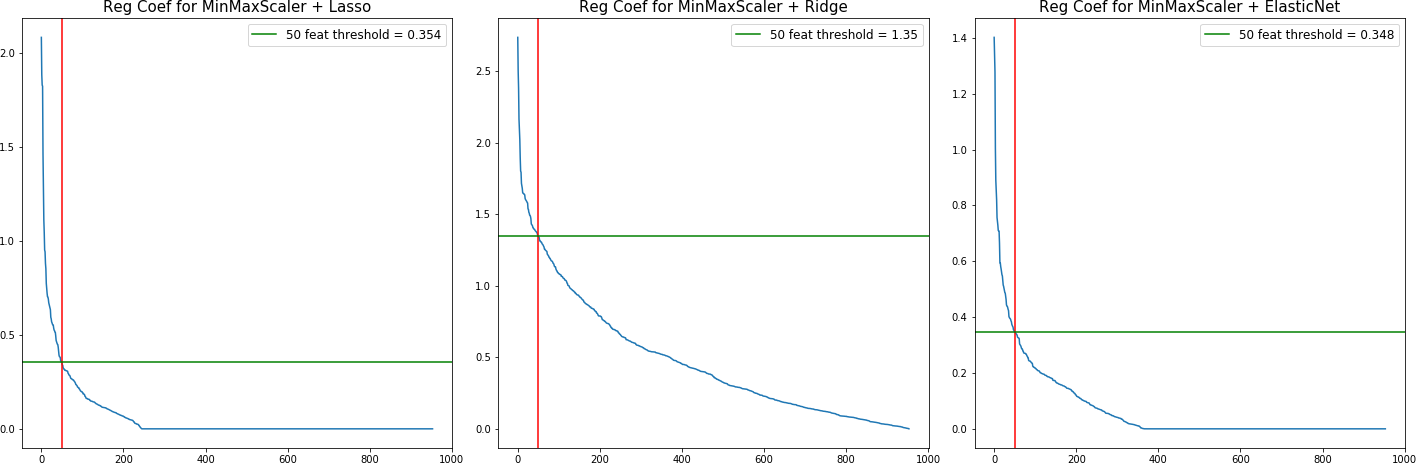
\includegraphics[width=\textwidth]{one_set_coefs.png}
	\caption{The three plots above show the three coefficients sets obtained through the three regression method on the whole dataset after the MinMax regularization. The values have been sorted by absolute value. The \textcolor{red}{red} vertical line shows the cut over the first 50 features. The \textcolor{ForestGreen}{green}  horizontal line detect the value of the 50$^{th}$ coefficient. In all of the three curves it's evident the \emph{elbow} behave of the curve and that the \emph{TOP 50} features cut falls around the elbow point.}
	\label{fig:3_coef}
	\centering
\end{figure}

\paragraph{Dimensionality Reduction}

From the silhouette of the curves in Figure \ref{fig:3_coef} it's clear the presence of an \textbf{\emph{elbow}}: a point where the curve starts decreasing more gently. That point was taken as \emph{reference} for the number of features to select from the whole set. The idea under this choice is that considering features beyond the elbow point pay less and less back respect to those feature before this point.

The coefficients form different regressors live in different value range, so I devised a \emph{non parametric} comparison method to score the features. The method is not based on the value of a feature's coefficient but on its \emph{position} in the sorted (by absolute value) array. As a score for each feature it was made a count of how frequent every feature appears in the top ranked in the different charts given by the different regression methods.

\paragraph{Example - \emph{Brain Challenge}}
The \emph{Brain Challenge}'s dataset contains around 1000 features (i.e. 954 numerical values). After the prior regressions the nine sets of coefficients were procured (three of which are shown in Figure \ref{fig:3_coef}). The precise detection of the \emph{elbow} point it's not a trivial task, so in a first phase of the project it was detected by eye to be around the 50$^{th}$ sorted features for each one of the values sets. This way it was possible to give a point to each features when it fell in the \emph{TOP 50} sorted set. The same exact process was repeated for smaller sets of features, in this case for the \emph{TOP 25} and the \emph{TOP 10}. A brief snapshot of the classification obtained follows below (a more detailed list in  Appendix \ref{sec:app1})

\begin{table}[ht]
\begin{tabular}{llll}
Feature Name                                        & TOP50 scores & TOP25 scores & TOP10 scores \\
\textit{Left.Putamen}                               & 9             & 9             & 9             \\
\textit{Left.Thalamus.Proper}                       & 9             & 9             & 9             \\
\textit{lh\_superiorfrontal\_thickness}             & 9             & 9             & 6             \\
\textit{X3rd.Ventricle}                             & 9             & 9             & 6             \\
\textit{Left.Cerebellum.Cortex}                     & 9             & 6             & 6             \\
\dots																								& \dots					&\dots 					&\dots
\end{tabular}
\end{table}



\section*{Regression on the Reduced Dataset}
In order to \emph{test} the quality of the dimensionality reduction a further regression should be performed both on the whole dataset and on the reduced ones. This time the restriction to linear models it's not necessary, indeed suport vector regressors and gaussian process were widely used too.

Those new regressors have been trained on the majority of the available dataset (around the 90\%) to predict the well known target value. Once trained, every regressor processes the remaining part of the dataset and make a prediction on the target values. Those predicted values are then put in comparison with the true ones with a straightforward linear model fitting. The $R^2$ score of that last fitting serves as \emph{quality score} of the regression on the reduction features space. This very quality score was used to quantify the change in performance of the same regressor on different reductions of the same feature space.

The detailed description of two different applications of this pipeline follows: both the faced dataset were made of biomedical data and allow the prediction of the age of the surveyed.



\section*{1$^{st}$ Application - \emph{Brain Challenge}}
\paragraph{The Dataset}
The dataset available for this analysis is a collection of 954 numerical features collected from NMR images of the brain of different patients in different sites, and 5 further categorical features that provide personal information of the surveyed like age, gender and the site of medical analysis. The aim of the analysis was to put in relation those numerical features with the age of the patients. In Figure \ref{fig:gend_distr} is shown the distribution among gender and age in the 16 different sites of analysis.

\begin{figure}[ht]
	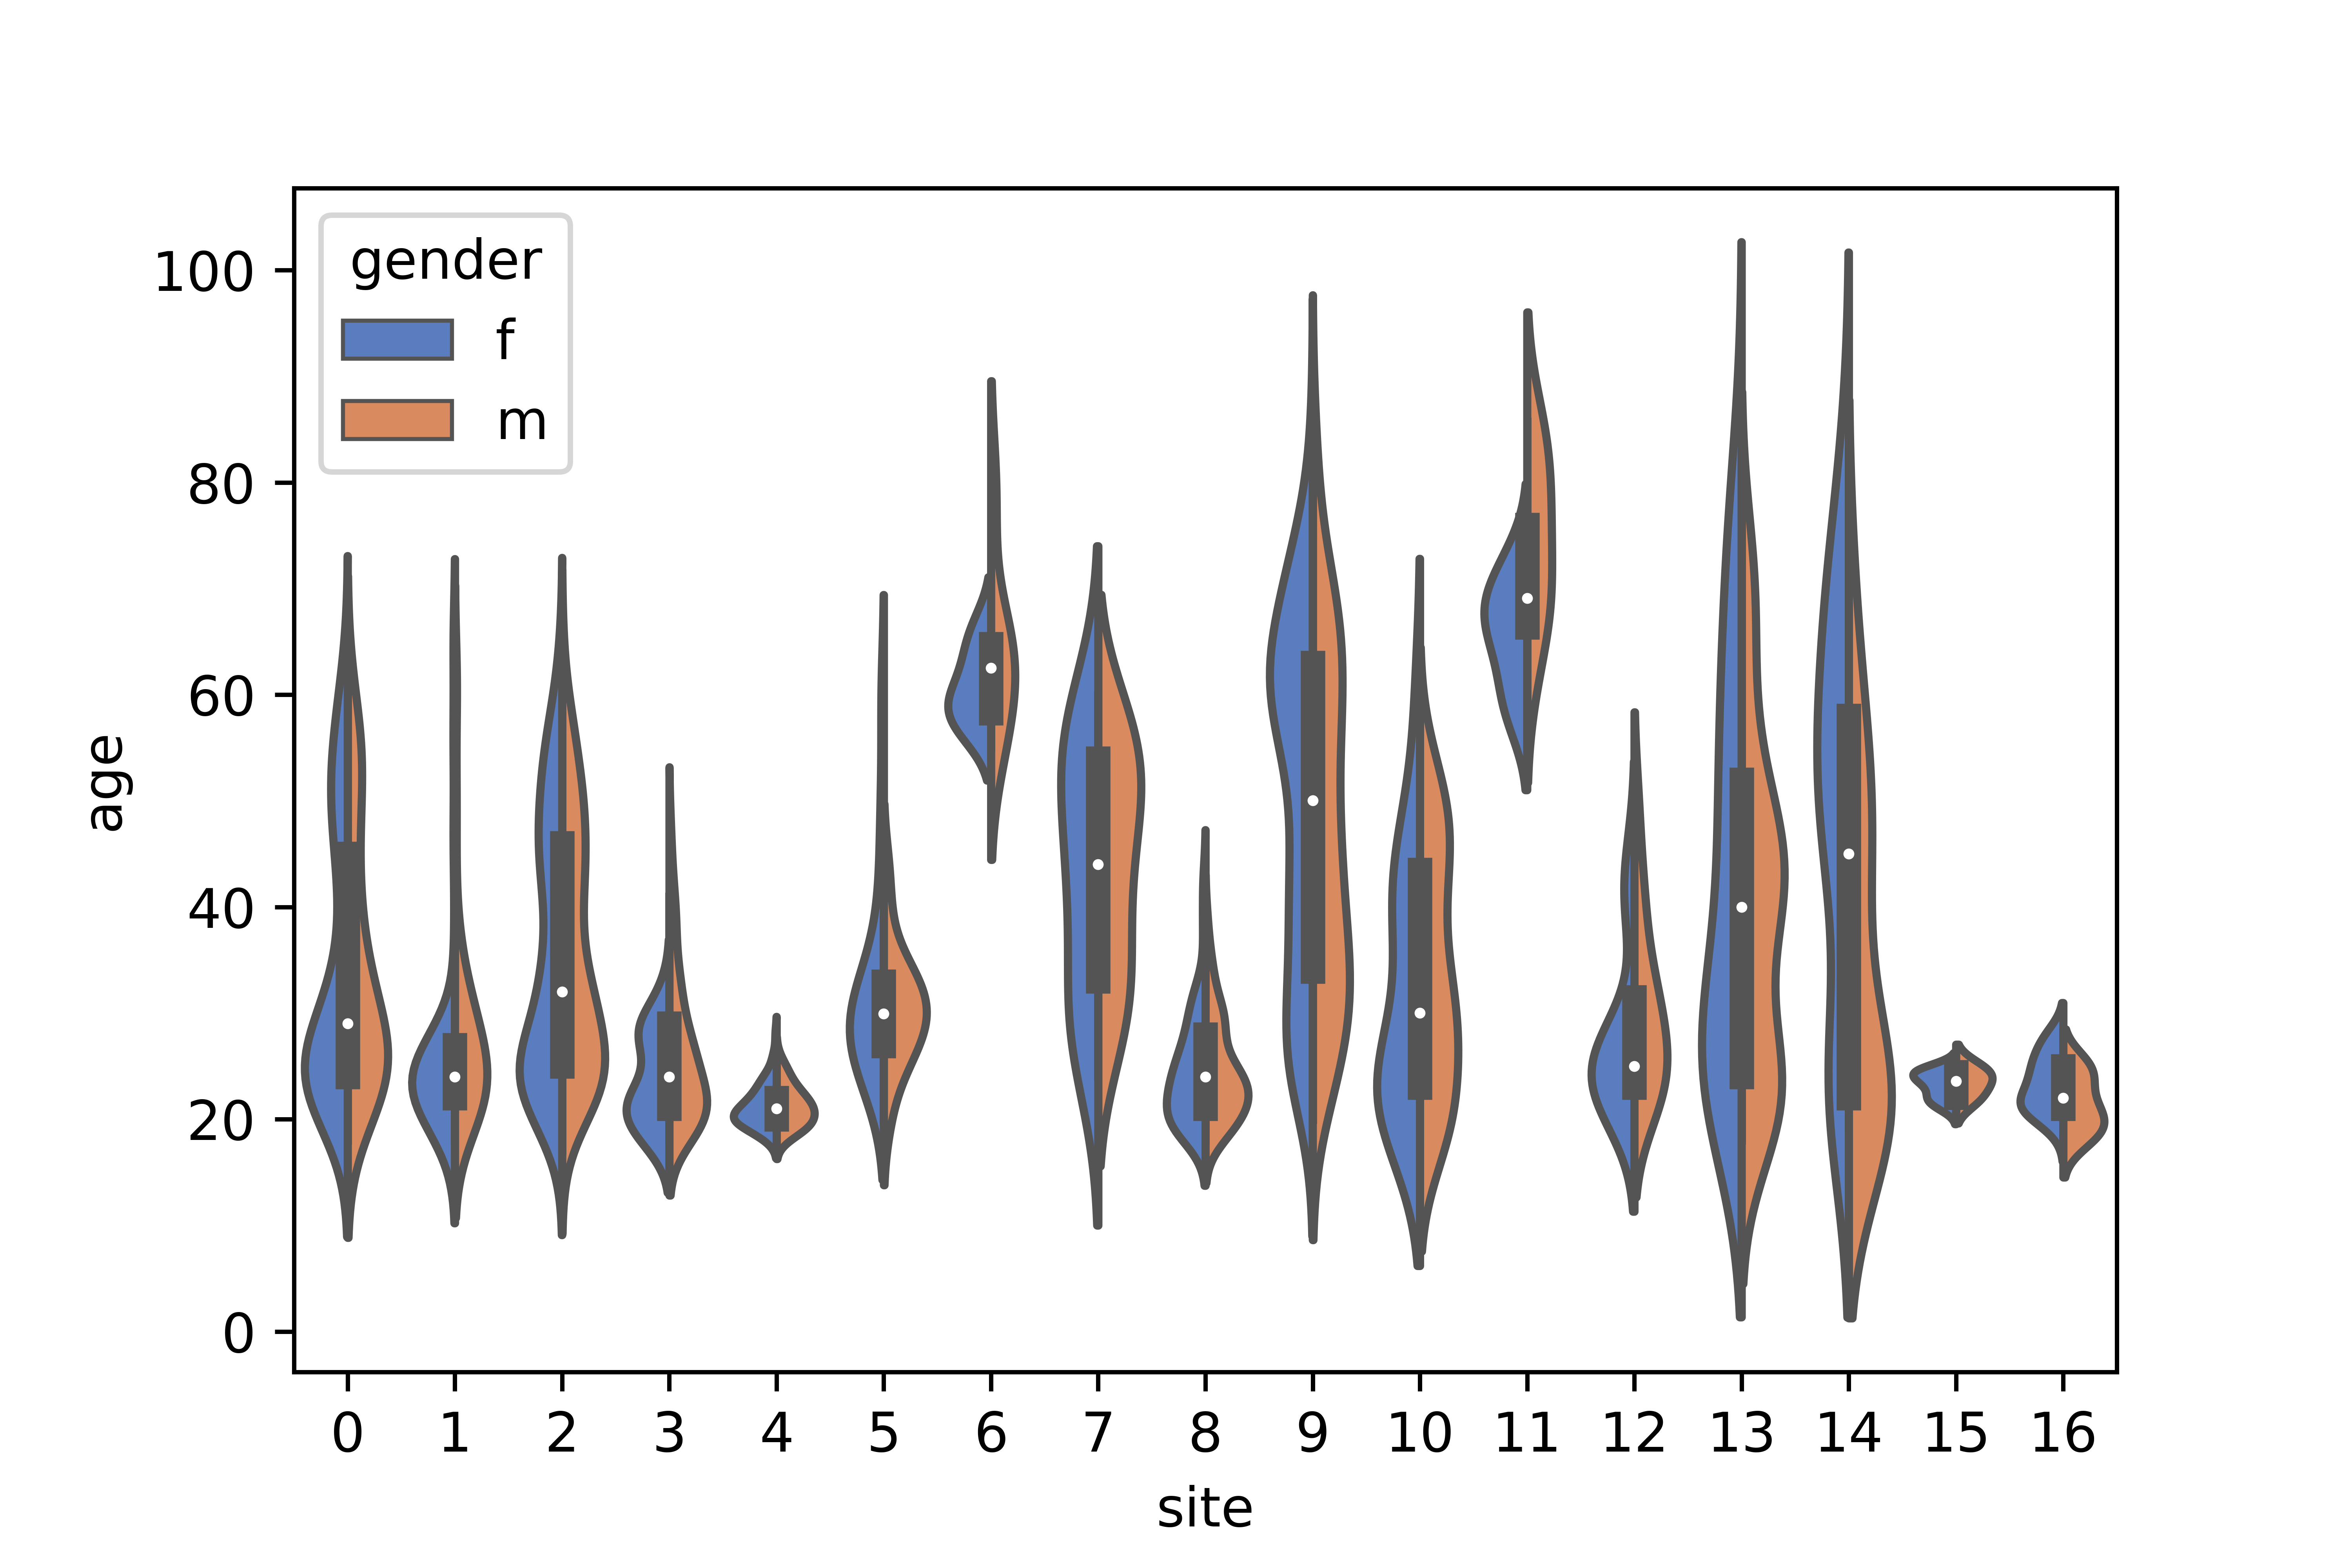
\includegraphics[width=\textwidth]{violin_gender_site}
	\caption{Series of violin graphs that show the distribution in gender and age among all the site of analysis. It turned out a clear majority of young surveyed of age around 20 years respect to the more grown, and only 3 or 4 sites cover homogeneously a wide range of age. The distribution between male and female instead appears to be quite symmetrical for each site.  }
	\label{fig:gend_distr}
	\centering
\end{figure}

\paragraph{Dimensionality Reduction}
Has previously stated, as can be seen in Figure \ref{fig:3_coef}, the elbow point for these 9 sets of coefficients fell around the 50$^{th}$ features. So three different selection were made; counting those features that appeared in the \emph{TOP 50}, in the \emph{TOP 25} and in the \emph{TOP 10} features of every set of regression coefficients. The complete list of features with the three kinds of scores is attached in Appendix \ref{sec:app1}.

\paragraph{Regression on Reduced Dataset}
In order to test the dimensionality reduction efficacy I performed as described above a further regression, using a Support Vector Regression (SVR) algorithm. The three reduction that were employed were the dataset containing all and only the 98 features that appeared at least once in a coefficient \emph{TOP 50}, the 49 appeared in the \emph{TOP 25} and the 18 appeared in the \emph{TOP 10}.
The SVR was trained on these dataset through a cross validated grid agorithm, that allows to scearch directly for those parameter that better fit the samples. The three different age predictions on the three dataset were put in relation with the true test values with a simple linear fitting, and a $R^2$ score were computed. In Figure \ref{fig:Brain_graphs} those three fitting are shown.

\begin{figure}[ht]
	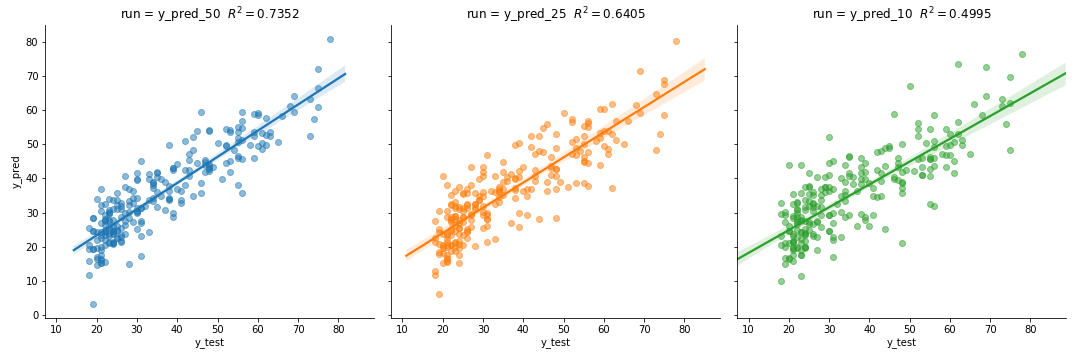
\includegraphics[width=\textwidth]{three_graphs}
	\caption{These are the three $R^2$ score obtained training the SVR on three different reductions of the feature space: selecting only those features that fell at least once in the \emph{TOP 50}, \emph{TOP 25} and \emph{TOP 10}. It's easy to see that reducing the dimension of the space the $R^2$ value drops. It's interesting seeing how a reduction in dimension from 954 to 98 (an order of magnitude) could anyway provide such a good $R^2$ score, around 0.74.}
	\label{fig:Brain_graphs}
	\centering
\end{figure}

In the plots in Figure \ref{fig:Brain_graphs} those $R^2$ score are reported. It's easy to see that reducing the dimension of the space the $R^2$ value drops. The first linear fit it's the one relative to the reduction in dimension to the most important 98 features. The $R^2$ score of that prediction is quite good (.ca 0.74). The successive two plot instead represent two more strict reduction to 49 and 18 features, in these cases the $R^2$ score drops coherently with the reduction.

It's interesting seeing how a reduction in dimension from 954 to 98 (a solid order of magnitude) could anyway provide such a good $R^2$ score, around 0.74. These behaviors have been considered as good hints of the correct work of this pipeline for the dimensionality reduction.

\section*{2$^{nd}$ Application - \emph{Cardiological Data}}

\paragraph{The Dataset} The dataset available for this analysis is a collection of around 2122 samples and 83 features. Only 72 of the features are numerical, the other are made of categorical value and more complex ones. Also in this case the aim of the analysis was the age prediction starting from the data.

\begin{figure}[ht]
	\centerline{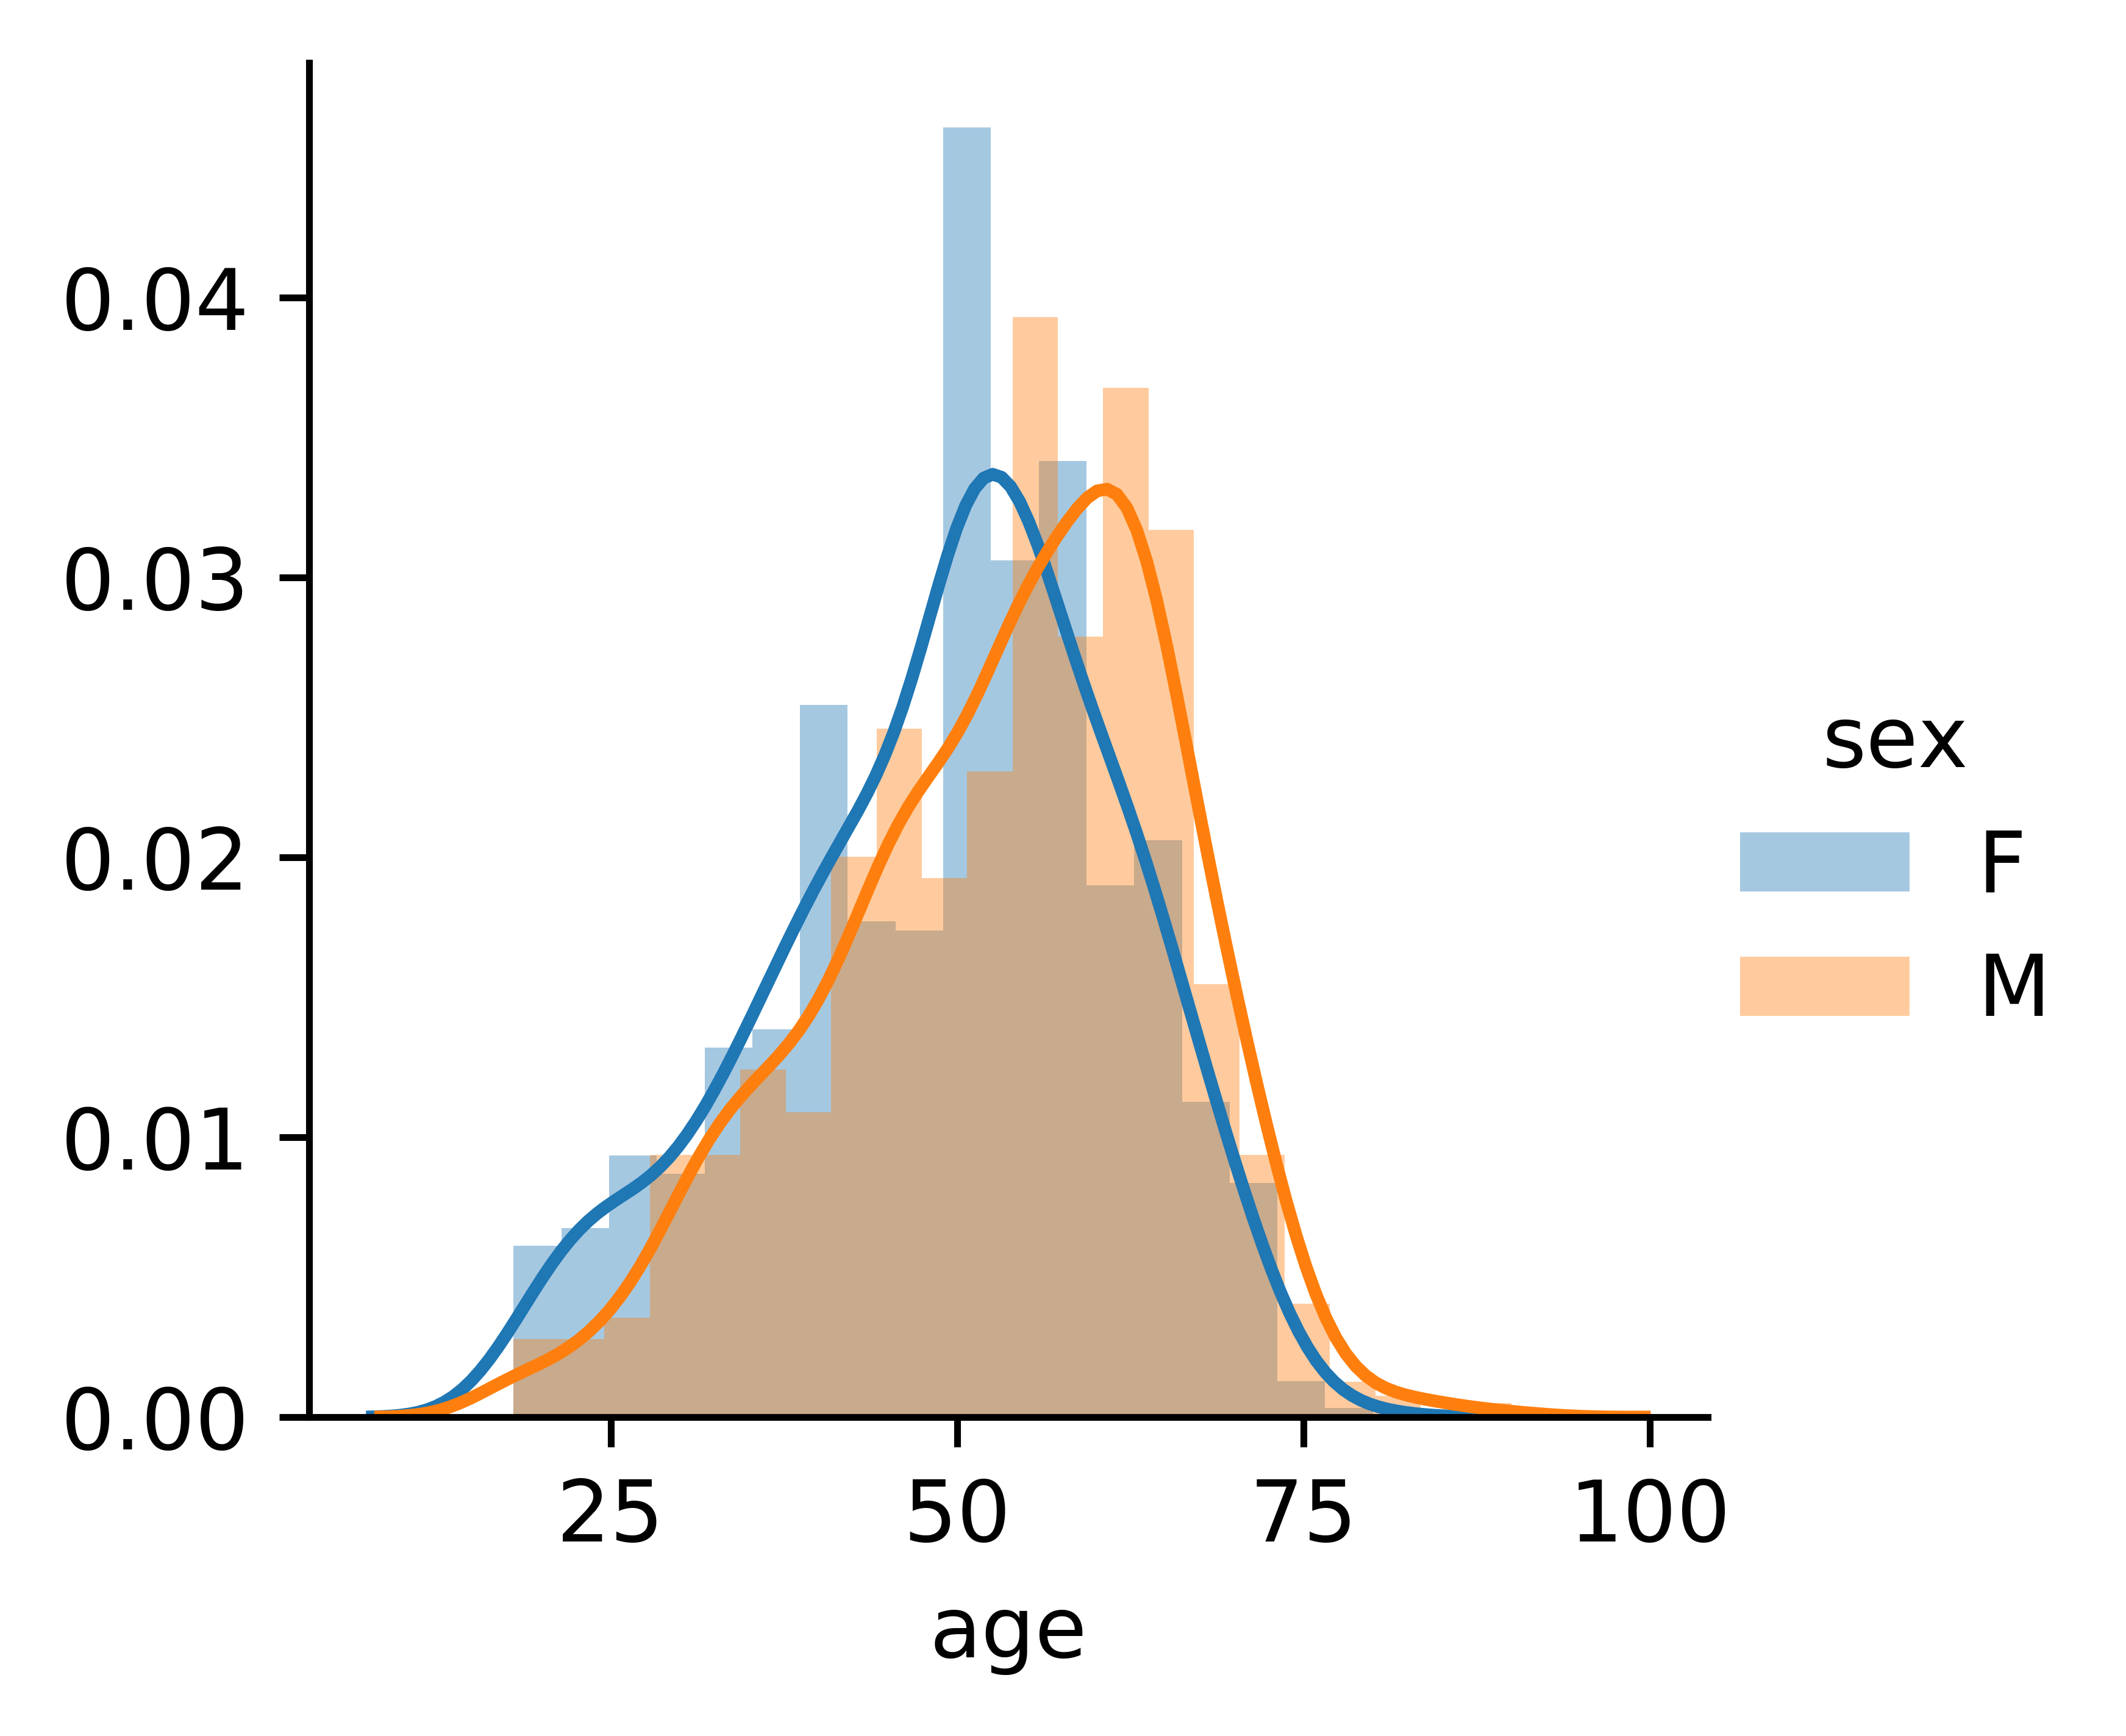
\includegraphics[width=0.6\textwidth]{Cardio_distribution}}
	\caption{ In this dataseta the distribution among ages between gender is quite similar. It generally seems an homogeneous survey.}
	\label{fig:cardio_distr}
	\centering
\end{figure}


\paragraph{Dimensionality Reduction} Almost all the consideration made previously for the Brain Challenge application hold here: the sorted coefficients presented all an elbow point around the 15$^{th}$ feature. Three cuts were made here as well detecting the \emph{TOP 20}, \emph{TOP 10} and \emph{TOP 5} in every set of coefficient. The list of the most important features according this method is shown in Appendix \ref{sec:app2}.

\paragraph{Regression on Reduced Dataset} The \emph{a posteriori} regression in this case was made with a Gaussian Process Regressor (GPR). This regressor was trained four independent times with the whole dataset and with the three reduced dataset according to the \emph{TOP 20} (23 features), \emph{TOP 10} (12 features)  and \emph{TOP 5} (5 features). Also this time the algorithm used for the training acted in a cross validated way searching for the best parameter. The four sets of predicted ages were put in comparison with the true values and the $R^2$ score computed (Figure \ref{fig:Cardio_graphs}).

\begin{figure}[ht]
	\centerline{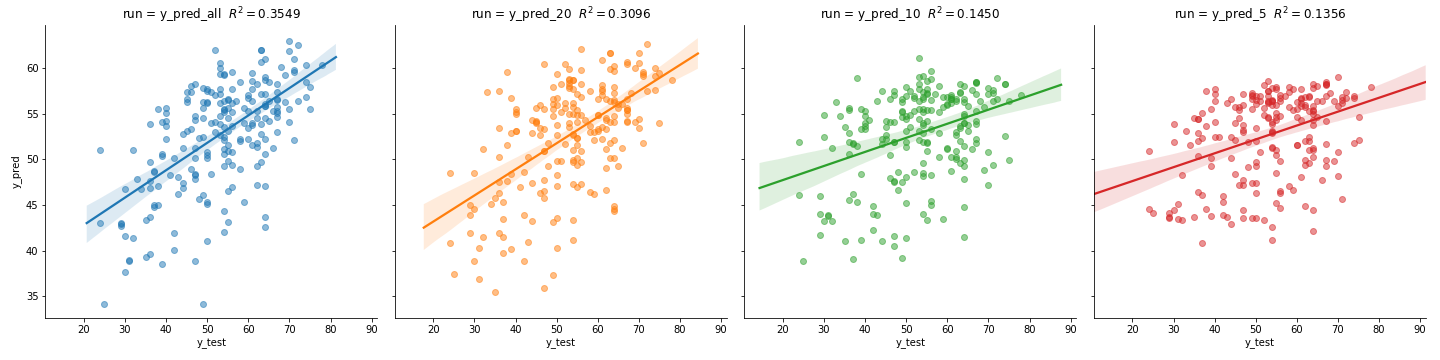
\includegraphics[width=1.3\textwidth]{four_graphs}}
	\caption{These are the three $R^2$ score obtained training the GPR on four different reductions of the feature space: selecting the whole dataset and those features that fell at least once in the \emph{TOP 20}, \emph{TOP 10} and \emph{TOP 5}. It's easy to see that reducing the dimension of the space the $R^2$ value drops. It's interesting to see how the reduction in dimension from the whole dataset (72 features) to the 23 features in the \emph{TOP 20} slightly reduces the score from 0.35 to 0.31. A further reduction instead sharply reduces the score.}
	\label{fig:Cardio_graphs}
	\centering
\end{figure}

In the plots shown in Figure \ref{fig:Cardio_graphs} it's possible to see the same behaviour of the $R^2$ score as in the 1$^{st}$ application: the more the feature space is reduced the more the score drops. It's interesting to see how the reduction in dimension from the whole dataset (72 features) to the 23 features in the \emph{TOP 20} slightly reduces the score from 0.35 to 0.31, a further reduction instead sharply reduces the score. This particular behavior strengthen the belief in the the efficacy of the algorithm for the dimensionality reduction.



\section*{Used Material}
In order to read and analyze the data for this project it was used exclusively \texttt{Python} code. In particular for reading and manipulating dataframe the library \texttt{Pandas}, for visualizing the results the library \texttt{Seaborn} and for the computing parts mainly the library \texttt{SciKitLeaern}.
In particular:

\begin{itemize}
	\item for the regularization:\texttt{ MinMaxScaler, StandardScaler, RobustScaler}
	\item for the penalized regressions: \texttt{ ElasticNetCV, LassoCV, RidgeCV}
	\item for the further regressions: \texttt{GaussianProcessRegressor, SVR}
	\item for searching the best parameters: \texttt{GridSearchCV}
\end{itemize}

and a lot of other tools from that library.

\newpage
\section*{Appendix 1 - Brain Challenge Features Charts} \label{sec:app1}
A more extended but not complete list of the most important features (they're .ca 200).
\begin{table}[ht]
\begin{tabular}{llll}
Feature Name                                        & TOP50 scores & TOP25 scores & TOP10 scores    \\
\textit{Left.Putamen}                               & 9             & 9             & 9             \\
\textit{Left.Thalamus.Proper}                       & 9             & 9             & 9             \\
\textit{lh\_superiorfrontal\_thickness}             & 9             & 9             & 6             \\
\textit{X3rd.Ventricle}                             & 9             & 9             & 6             \\
\textit{Left.Cerebellum.Cortex}                     & 9             & 6             & 6             \\
\textit{Right.Lateral.Ventricle}                    & 6             & 6             & 6             \\
\textit{lh\_G\_front\_sup\_thickness}               & 6             & 6             & 6             \\
\textit{lh\_S\_circular\_insula\_inf\_thicknessstd} & 6             & 6             & 6             \\
\textit{Brain.Stem}                                 & 6             & 6             & 6             \\
\textit{Right.Amygdala}                             & 6             & 6             & 6             \\
\textit{rh\_G\_front\_sup\_thickness}               & 6             & 6             & 3             \\
\textit{lh\_Pole\_occipital\_thickness}             & 9             & 6             & 0             \\
\textit{lh\_WhiteSurfArea\_area}                    & 9             & 6             & 0             \\
\textit{lh\_S\_precentral.sup.part\_thickness}      & 6             & 6             & 0             \\
\textit{X4th.Ventricle}                             & 6             & 6             & 0             \\
\textit{rh.fimbria}                                 & 6             & 6             & 0             \\
\textit{BrainSegVol.to.eTIV}                        & 6             & 6             & 0             \\
\textit{Right.VentralDC}                            & 6             & 6             & 0             \\
\textit{lh\_S\_circular\_insula\_sup\_thicknessstd} & 6             & 6             & 0             \\
\textit{rh\_parsopercularis\_thicknessstd}          & 6             & 6             & 0             \\
\textit{rh\_S\_subparietal\_area}                   & 6             & 6             & 0             \\
\textit{lh\_posteriorcingulate\_area}               & 6             & 6             & 0
\end{tabular}
\end{table}

\newpage
\section*{Appendix 2 - Cardiological Data Features Charts} \label{sec:app2}
The complete list of the most important features.
\begin{table}[ht]
\begin{tabular}{llll}
Feature Name       & TOP20 scores  & TOP10 scores  & TOP5 scores \\
\textit{ac\_slope} & 9             & 9             & 9            \\
\textit{ad\_slope} & 9             & 9             & 9            \\
\textit{sdsd}      & 9             & 9             & 9            \\
\textit{smoke}     & 9             & 9             & 9            \\
\textit{rmssd}     & 9             & 9             & 9            \\
\textit{t\_ad}     & 9             & 9             & 0            \\
\textit{bc\_slope} & 9             & 9             & 0            \\
\textit{ibi}       & 9             & 9             & 0            \\
\textit{t\_bd}     & 9             & 6             & 0            \\
\textit{t\_ac}     & 9             & 6             & 0            \\
\textit{afib}      & 9             & 3             & 0            \\
\textit{tpr}       & 9             & 3             & 0            \\
\textit{dt\_var}   & 9             & 0             & 0            \\
\textit{bd\_slope} & 9             & 0             & 0            \\
\textit{sdnn}      & 9             & 0             & 0            \\
\textit{b}         & 9             & 0             & 0            \\
\textit{c}         & 9             & 0             & 0            \\
\textit{AGI}       & 9             & 0             & 0            \\
\textit{ae\_slope} & 6             & 0             & 0            \\
\textit{pnn50}     & 6             & 0             & 0            \\
\textit{b - (d/a)} & 3             & 0             & 0            \\
\textit{pnn20}     & 3             & 0             & 0
\end{tabular}
\end{table}

\end{document}
